% arara: pdflatex: {files: [MathSACpr2014]}
\chapter{Other  Curricular Issues}
\section[Distance education]{To what degree are courses offered in a Distance modality (on-line, hybrid, interactive television, etc)? For courses offered both via DL and on-campus, are there differences in student success? (Contact the Office of Institutional Effectiveness , either Laura Massey or Rob Vergun,  for course-level data). If so, how are you, or will you address these differences? What significant revelations, concerns or questions arise in the area of DL delivery?}

\subsection{Presence of DL offerings}
The Math SAC offers Distance Learning (DL) courses in on-line, hybrid, and interactive television (ITV) modalities.  We strive to make our DL course experience simulate the face-to-face course experience with respect to instructor presence, feedback, and assessment. We use discussion boards to simulate the classroom learning environment, and an array of online homework platforms to assess and prepare our students effectively. A Math SAC DL standing committee is charged with discussing the structure of our current DL courses, as well as developing and maintaining current DL best practices and standards.

All of our pre-college level math courses (except a calculator skills course) have a DL offering, as do most of our lower-division collegiate courses.  Courses that are not offered using a distance modality fall into two categories: those on the high end of our collegiate courses, and specialty courses with low enrollments. See \cref{tab:sec3:DLofferings}.

\begin{table}
\caption{Course Offerings through Distance Learning}\label{tab:sec3:DLofferings}
\centering
\begin{tabular}{ccccccccc}
\toprule
\multicolumn{3}{p{1in}}{Offered as DL} & \multicolumn{3}{p{1in}}{Not offered  DL upper division} & \multicolumn{3}{p{1in}}{Not offered  DL specialty}\\
\midrule
020& 030& 060& 		251& 252& 253&		015& 25C& 26C\\
065& 070& 084& 		254& 256& 261&		061& 062& 063\\
095& 111& 112& 		&&&					093& 105& 211\\
241& 243& 244&		&&&					212& 213\\

\bottomrule
\end{tabular}
\end{table}

Approximately 14.1\% of PCC math enrollments were into a DL class during the academic year of 2012/13 compared to only 9.1\% in the 2007/08 academic year. This percentage increase is coupled with a general enrollment surge over the past five years, and the number of DL enrollments has grown by over 150\% in this time period. \Cref{fig:sec3:DLenrollments,fig:sec3:F2Fenrollments} show student enrollment in face-to-face courses compared to online courses over six academic years. Note that even while overall enrollment has declined some since its peak in 2011/12, that absolute enrollment in DL courses has still grown. \Cref{tab:sec3:F2FandDLdata} gives more detailed data.

\begin{figure}[!htb]
    \begin{minipage}{.5\textwidth}
          %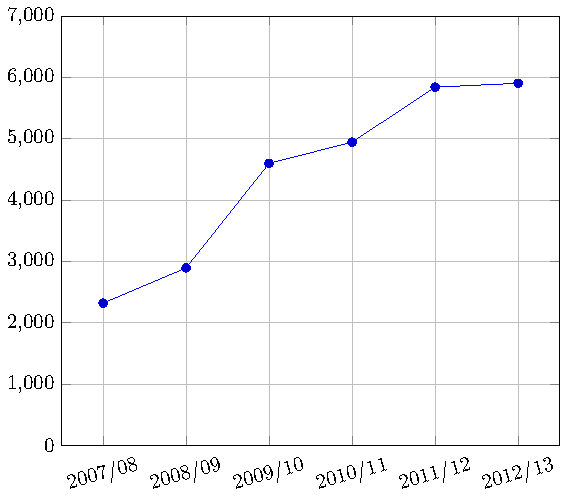
\includegraphics[width=\textwidth]{graphics/enrollmentInDL.pdf}
          % arara: pdflatex
% !arara: indent: {overwrite: yes}
\documentclass{standalone}
% Caption: Enrollment in DL
% 2007/08-2012/13

\usepackage{pgfplots}
\usepackage{pgfplotstable}
\pgfplotsset{compat=newest}


\begin{document}

% http://tex.stackexchange.com/questions/128468/problems-with-pgfplotstableread-and-relative-paths
\IfStandalone{
	\newcommand{\fromRoot}[1]{../data/#1}
	}{
	\newcommand{\fromRoot}[1]{./data/#1}
}

% need to have the read command in the main document, otherwise it will 
% be ignored when used with standalone
\pgfplotstableread[col sep=comma]{\fromRoot{ProcessedGradesData.csv}}\enrollmentdata

\begin{tikzpicture}
	\begin{axis}[
			%ybar,
			symbolic x coords={2007/08, 2008/09, 2009/10, 2010/11, 2011/12, 2012/13, NaN},
			xtick=data,
			minor ytick={1000,2000,...,7000},
			enlarge x limits,
			%scale only axis,       
			grid = both,
			ymin=0,ymax=7000,
			scaled ticks=false, 
			tick label style={/pgf/number format/fixed},
			legend pos=outer north east,
			restrict x to domain=0:5,
			x tick label style={rotate=25},
			width=\textwidth,
		]
		\addplot table[x=AY,y=DL_Enrollments]{\enrollmentdata};
		%\legend{DL}
	\end{axis}
\end{tikzpicture}
\end{document}

          \caption{Enrollments in DL}\label{fig:sec3:DLenrollments}
    \end{minipage}%
    \begin{minipage}{.5\textwidth}
          %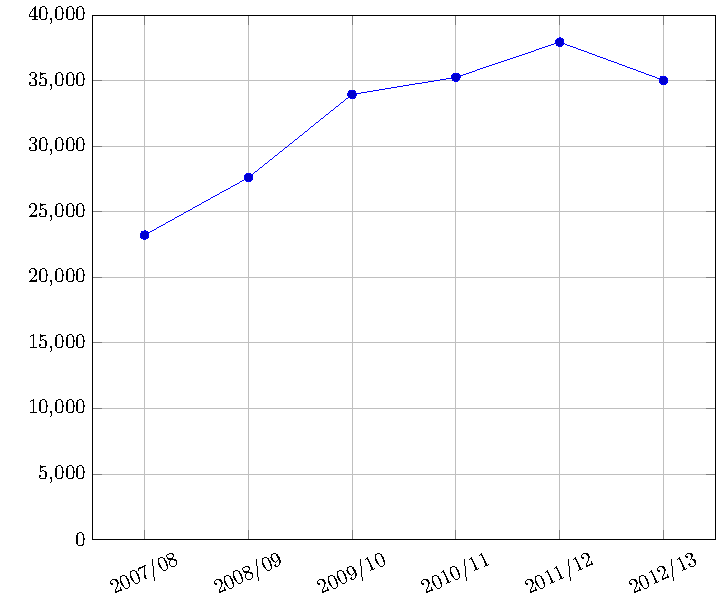
\includegraphics[width=\textwidth]{graphics/enrollmentInF2F.pdf}
          % arara: pdflatex
% !arara: indent: {overwrite: yes}
\documentclass{standalone}
% Caption: Enrollment in F2F
% 2007/08-2012/13

\usepackage{pgfplots}
\usepackage{pgfplotstable}
\pgfplotsset{compat=newest}

\pgfplotstableread[col sep=comma]{../data/ProcessedGradesData.csv}\enrollmentdata

\begin{document}

\begin{tikzpicture}
	\begin{axis}[
			%ybar,
			symbolic x coords={2007/08, 2008/09, 2009/10, 2010/11, 2011/12, 2012/13, NaN},
			xtick=data,
			%minor ytick={1000,5000,...,40000},
			enlarge x limits,
			scale only axis,       
			grid = both,
			ymin=0,ymax=40000,
			scaled ticks=false, 
			tick label style={/pgf/number format/fixed},
			legend pos=outer north east,
			restrict x to domain=0:5,
			x tick label style={rotate=15},
		]
		\addplot table[x=AY,y=F2F_Enrollments]{\enrollmentdata};
		%\legend{DL}
	\end{axis}
\end{tikzpicture}
\end{document}

          \caption{Enrollments in F2F}\label{fig:sec3:F2Fenrollments}
    \end{minipage}
\end{figure}

\begin{sidewaystable}
  	\caption{DL/F2F enrollments and pass rates}\label{tab:sec3:F2FandDLdata}
	\centering
	\begin{minipage}{\textwidth}
          % arara: pdflatex
\documentclass[varwidth]{standalone}
\usepackage{pgfplotstable}
\usepackage{booktabs}
\usepackage{multirow}

% caption: pass rates by class for DL vs F2F 2007-2008

% empty column type- very useful
\newcolumntype{H}{>{\setbox0=\hbox\bgroup}c<{\egroup}@{}}

\pgfplotstableset{percentstyle/.style={
    preproc/expr={##1*100},
    dec sep align,fixed,fixed zerofill,
postproc cell content/.append code={
            \ifx\\##1\\% check if ##1 is empty
            \else
            \ifnum1=\pgfplotstablepartno
                \pgfkeysalso{@cell content/.add={}{\,\%}}%
            \fi
            \fi
        },
    precision=0,
}
}

% references:
%   http://tex.stackexchange.com/questions/65760/pgfplotstable-how-can-i-add-percent-signs-and-respect-dec-sep-align
%   http://tex.stackexchange.com/questions/16604/easiest-way-to-delete-a-column/16607#16607
%   http://tex.stackexchange.com/questions/89365/check-for-empty-macro-argument

\begin{document}

% http://tex.stackexchange.com/questions/128468/problems-with-pgfplotstableread-and-relative-paths
\IfStandalone{
	\newcommand{\fromRoot}[1]{../data/#1}
	}{
	\newcommand{\fromRoot}[1]{./data/#1}
}

\pgfplotstableread[col sep=comma]{\fromRoot{dlvsF2FenrollmentPassRates.csv}}\dlvsftofdata

\pgfplotstabletypeset[
every head row/.style={
        before row={%
        \toprule
        \multirow{2}{*}{Course}
        & \multicolumn{7}{c}{2007--2008} 
        & \multicolumn{7}{c}{2008--2009} 
        & \multicolumn{22}{c}{2009--2010} 
        \\},
        after row=\midrule},
every last row/.style={after row=\bottomrule},
columns/Course/.style={string type,column name={},column type=r},
    % 2007-08
    % 2007-08
    % 2007-08
    columns/2007-08/.style={column type=H},
    columns/DL2007-08/.style={column name={DL},column type=r},
    columns/DL Pass rate2007-08/.style={column name={\% Pass},percentstyle},
    columns/FtoF2007-08/.style={column name={F2F},column type=r},
    columns/FtoF Pass rate2007-08/.style={column name={\% Pass},percentstyle},
    % 2008-09
    % 2008-09
    % 2008-09
    columns/2008-09/.style={column type=H},
    columns/DL2008-09/.style={column name={DL},column type=r},
    columns/DL Pass rate2008-09/.style={column name={\% Pass},percentstyle},
    columns/FtoF2008-09/.style={column name={F2F},column type=r},
    columns/FtoF Pass rate2008-09/.style={column name={\% Pass},percentstyle},
    % 2009-10
    % 2009-10
    % 2009-10
    columns/2009-10/.style={column type=H},
    columns/DL2009-10/.style={column name={DL},column type=r},
    columns/DL Pass rate2009-10/.style={column name={\% Pass},percentstyle},
    columns/FtoF2009-10/.style={column name={F2F},column type=r},
    columns/FtoF Pass rate2009-10/.style={column name={\% Pass},percentstyle},
    % 2010-11
    % 2010-11
    % 2010-11
    columns/2010-11/.style={column type=H},
    columns/DL2010-11/.style={column type=H},
    columns/DL Pass rate2010-11/.style={column type=H},
    columns/FtoF2010-11/.style={column type=H},
    columns/FtoF Pass rate2010-11/.style={column type=H},
    % 2011-12
    % 2011-12
    % 2011-12
    columns/2011-12/.style={column type=H},
    columns/DL2011-12/.style={column type=H},
    columns/DL Pass rate2011-12/.style={column type=H},
    columns/FtoF2011-12/.style={column type=H},
    columns/FtoF Pass rate2011-12/.style={column type=H},
    % 2012-13
    % 2012-13
    % 2012-13
    columns/2012-13/.style={column type=H},
    columns/DL2012-13/.style={column type=H},
    columns/DL Pass rate2012-13/.style={column type=H},
    columns/FtoF2012-13/.style={column type=H},
    columns/FtoF Pass rate2012-13/.style={column type=H},
    % ignore these columns
    columns/2008-09/.style={column type=H},
    columns/2009-10/.style={column type=H},
    columns/2010-11/.style={column type=H},
    columns/2011-12/.style={column type=H},
    columns/2012-13/.style={column type=H},
]{\dlvsftofdata}

\end{document}

          \vspace{2pc}
          % arara: pdflatex
\documentclass[varwidth]{standalone}
\usepackage{pgfplotstable}
\usepackage{booktabs}
\usepackage{multirow}

% caption: pass rates by class for DL vs F2F 2010-2013

% empty column type- very useful
\newcolumntype{H}{>{\setbox0=\hbox\bgroup}c<{\egroup}@{}}

\pgfplotstableset{percentstyle/.style={
    preproc/expr={##1*100},
    dec sep align,fixed,fixed zerofill,
postproc cell content/.append code={
            \ifx\\##1\\% check if ##1 is empty
            \else
            \ifnum1=\pgfplotstablepartno
                \pgfkeysalso{@cell content/.add={}{\,\%}}%
            \fi
            \fi
        },
    precision=0,
}
}

% references:
%   http://tex.stackexchange.com/questions/65760/pgfplotstable-how-can-i-add-percent-signs-and-respect-dec-sep-align
%   http://tex.stackexchange.com/questions/16604/easiest-way-to-delete-a-column/16607#16607
%   http://tex.stackexchange.com/questions/89365/check-for-empty-macro-argument

\begin{document}

% http://tex.stackexchange.com/questions/128468/problems-with-pgfplotstableread-and-relative-paths
\IfStandalone{
	\newcommand{\fromRoot}[1]{../data/#1}
	}{
	\newcommand{\fromRoot}[1]{./data/#1}
}

\pgfplotstableread[col sep=comma]{\fromRoot{dlvsF2FenrollmentPassRates.csv}}\dlvsftofdata


\pgfplotstabletypeset[
every head row/.style={
        before row={%
        \toprule
        \multirow{2}{*}{Course}
        & \multicolumn{22}{c}{2010--2011} 
        & \multicolumn{7}{c}{2011--2012} 
        & \multicolumn{7}{c}{2012--2013} 
        \\},
        after row=\midrule},
every last row/.style={after row=\bottomrule},
columns/Course/.style={string type,column name={},column type=r},
    % 2007-08
    % 2007-08
    % 2007-08
    columns/2007-08/.style={column type=H},
    columns/DL2007-08/.style={column type=H},
    columns/DL Pass rate2007-08/.style={column type=H},
    columns/FtoF2007-08/.style={column type=H},
    columns/FtoF Pass rate2007-08/.style={column type=H},
    % 2008-09
    % 2008-09
    % 2008-09
    columns/2008-09/.style={column type=H},
    columns/DL2008-09/.style={column type=H},
    columns/DL Pass rate2008-09/.style={column type=H},
    columns/FtoF2008-09/.style={column type=H},
    columns/FtoF Pass rate2008-09/.style={column type=H},
    % 2009-10
    % 2009-10
    % 2009-10
    columns/2009-10/.style={column type=H},
    columns/DL2009-10/.style={column type=H},
    columns/DL Pass rate2009-10/.style={column type=H},
    columns/FtoF2009-10/.style={column type=H},
    columns/FtoF Pass rate2009-10/.style={column type=H},
    % 2010-11
    % 2010-11
    % 2010-11
    columns/2010-11/.style={column type=H},
    columns/DL2010-11/.style={column name={DL},column type=r},
    columns/DL Pass rate2010-11/.style={column name={\% Pass},percentstyle},
    columns/FtoF2010-11/.style={column name={F2F},column type=r},
    columns/FtoF Pass rate2010-11/.style={column name={\% Pass},percentstyle},
    % 2011-12
    % 2011-12
    % 2011-12
    columns/2011-12/.style={column type=H},
    columns/DL2011-12/.style={column name={DL},column type=r},
    columns/DL Pass rate2011-12/.style={column name={\% Pass},percentstyle},
    columns/FtoF2011-12/.style={column name={F2F},column type=r},
    columns/FtoF Pass rate2011-12/.style={column name={\% Pass},percentstyle},
    % 2012-13
    % 2012-13
    % 2012-13
    columns/2012-13/.style={column type=H},
    columns/DL2012-13/.style={column name={DL},column type=r},
    columns/DL Pass rate2012-13/.style={column name={\% Pass},percentstyle},
    columns/FtoF2012-13/.style={column name={F2F},column type=r},
    columns/FtoF Pass rate2012-13/.style={column name={\% Pass},percentstyle},
    % ignore these columns
    columns/2008-09/.style={column type=H},
    columns/2009-10/.style={column type=H},
    columns/2010-11/.style={column type=H},
    columns/2011-12/.style={column type=H},
    columns/2012-13/.style={column type=H},
]{\dlvsftofdata}

\end{document}

          \end{minipage}
\end{sidewaystable}

\fixthis{I don't think these tables should be rotated- I liked them in a widepage- here's a working version, see what you think; make sure 
to put labels back on}
\begin{table}
	\begin{widepage}
	\centering
  	\caption{DL \& F2F enrollments and pass rates 2007--2010}%\label{tab:sec3:F2FandDLdata}
          % arara: pdflatex
\documentclass[varwidth]{standalone}
\usepackage{pgfplotstable}
\usepackage{booktabs}
\usepackage{multirow}

% caption: pass rates by class for DL vs F2F 2007-2008

% empty column type- very useful
\newcolumntype{H}{>{\setbox0=\hbox\bgroup}c<{\egroup}@{}}

\pgfplotstableset{percentstyle/.style={
    preproc/expr={##1*100},
    dec sep align,fixed,fixed zerofill,
postproc cell content/.append code={
            \ifx\\##1\\% check if ##1 is empty
            \else
            \ifnum1=\pgfplotstablepartno
                \pgfkeysalso{@cell content/.add={}{\,\%}}%
            \fi
            \fi
        },
    precision=0,
}
}

% references:
%   http://tex.stackexchange.com/questions/65760/pgfplotstable-how-can-i-add-percent-signs-and-respect-dec-sep-align
%   http://tex.stackexchange.com/questions/16604/easiest-way-to-delete-a-column/16607#16607
%   http://tex.stackexchange.com/questions/89365/check-for-empty-macro-argument

\begin{document}

% http://tex.stackexchange.com/questions/128468/problems-with-pgfplotstableread-and-relative-paths
\IfStandalone{
	\newcommand{\fromRoot}[1]{../data/#1}
	}{
	\newcommand{\fromRoot}[1]{./data/#1}
}

\pgfplotstableread[col sep=comma]{\fromRoot{dlvsF2FenrollmentPassRates.csv}}\dlvsftofdata

\pgfplotstabletypeset[
every head row/.style={
        before row={%
        \toprule
        \multirow{2}{*}{Course}
        & \multicolumn{7}{c}{2007--2008} 
        & \multicolumn{7}{c}{2008--2009} 
        & \multicolumn{22}{c}{2009--2010} 
        \\},
        after row=\midrule},
every last row/.style={after row=\bottomrule},
columns/Course/.style={string type,column name={},column type=r},
    % 2007-08
    % 2007-08
    % 2007-08
    columns/2007-08/.style={column type=H},
    columns/DL2007-08/.style={column name={DL},column type=r},
    columns/DL Pass rate2007-08/.style={column name={\% Pass},percentstyle},
    columns/FtoF2007-08/.style={column name={F2F},column type=r},
    columns/FtoF Pass rate2007-08/.style={column name={\% Pass},percentstyle},
    % 2008-09
    % 2008-09
    % 2008-09
    columns/2008-09/.style={column type=H},
    columns/DL2008-09/.style={column name={DL},column type=r},
    columns/DL Pass rate2008-09/.style={column name={\% Pass},percentstyle},
    columns/FtoF2008-09/.style={column name={F2F},column type=r},
    columns/FtoF Pass rate2008-09/.style={column name={\% Pass},percentstyle},
    % 2009-10
    % 2009-10
    % 2009-10
    columns/2009-10/.style={column type=H},
    columns/DL2009-10/.style={column name={DL},column type=r},
    columns/DL Pass rate2009-10/.style={column name={\% Pass},percentstyle},
    columns/FtoF2009-10/.style={column name={F2F},column type=r},
    columns/FtoF Pass rate2009-10/.style={column name={\% Pass},percentstyle},
    % 2010-11
    % 2010-11
    % 2010-11
    columns/2010-11/.style={column type=H},
    columns/DL2010-11/.style={column type=H},
    columns/DL Pass rate2010-11/.style={column type=H},
    columns/FtoF2010-11/.style={column type=H},
    columns/FtoF Pass rate2010-11/.style={column type=H},
    % 2011-12
    % 2011-12
    % 2011-12
    columns/2011-12/.style={column type=H},
    columns/DL2011-12/.style={column type=H},
    columns/DL Pass rate2011-12/.style={column type=H},
    columns/FtoF2011-12/.style={column type=H},
    columns/FtoF Pass rate2011-12/.style={column type=H},
    % 2012-13
    % 2012-13
    % 2012-13
    columns/2012-13/.style={column type=H},
    columns/DL2012-13/.style={column type=H},
    columns/DL Pass rate2012-13/.style={column type=H},
    columns/FtoF2012-13/.style={column type=H},
    columns/FtoF Pass rate2012-13/.style={column type=H},
    % ignore these columns
    columns/2008-09/.style={column type=H},
    columns/2009-10/.style={column type=H},
    columns/2010-11/.style={column type=H},
    columns/2011-12/.style={column type=H},
    columns/2012-13/.style={column type=H},
]{\dlvsftofdata}

\end{document}

          \vspace{2pc}
  	\caption{DL \& F2F enrollments and pass rates 2010--2013}
          % arara: pdflatex
\documentclass[varwidth]{standalone}
\usepackage{pgfplotstable}
\usepackage{booktabs}
\usepackage{multirow}

% caption: pass rates by class for DL vs F2F 2010-2013

% empty column type- very useful
\newcolumntype{H}{>{\setbox0=\hbox\bgroup}c<{\egroup}@{}}

\pgfplotstableset{percentstyle/.style={
    preproc/expr={##1*100},
    dec sep align,fixed,fixed zerofill,
postproc cell content/.append code={
            \ifx\\##1\\% check if ##1 is empty
            \else
            \ifnum1=\pgfplotstablepartno
                \pgfkeysalso{@cell content/.add={}{\,\%}}%
            \fi
            \fi
        },
    precision=0,
}
}

% references:
%   http://tex.stackexchange.com/questions/65760/pgfplotstable-how-can-i-add-percent-signs-and-respect-dec-sep-align
%   http://tex.stackexchange.com/questions/16604/easiest-way-to-delete-a-column/16607#16607
%   http://tex.stackexchange.com/questions/89365/check-for-empty-macro-argument

\begin{document}

% http://tex.stackexchange.com/questions/128468/problems-with-pgfplotstableread-and-relative-paths
\IfStandalone{
	\newcommand{\fromRoot}[1]{../data/#1}
	}{
	\newcommand{\fromRoot}[1]{./data/#1}
}

\pgfplotstableread[col sep=comma]{\fromRoot{dlvsF2FenrollmentPassRates.csv}}\dlvsftofdata


\pgfplotstabletypeset[
every head row/.style={
        before row={%
        \toprule
        \multirow{2}{*}{Course}
        & \multicolumn{22}{c}{2010--2011} 
        & \multicolumn{7}{c}{2011--2012} 
        & \multicolumn{7}{c}{2012--2013} 
        \\},
        after row=\midrule},
every last row/.style={after row=\bottomrule},
columns/Course/.style={string type,column name={},column type=r},
    % 2007-08
    % 2007-08
    % 2007-08
    columns/2007-08/.style={column type=H},
    columns/DL2007-08/.style={column type=H},
    columns/DL Pass rate2007-08/.style={column type=H},
    columns/FtoF2007-08/.style={column type=H},
    columns/FtoF Pass rate2007-08/.style={column type=H},
    % 2008-09
    % 2008-09
    % 2008-09
    columns/2008-09/.style={column type=H},
    columns/DL2008-09/.style={column type=H},
    columns/DL Pass rate2008-09/.style={column type=H},
    columns/FtoF2008-09/.style={column type=H},
    columns/FtoF Pass rate2008-09/.style={column type=H},
    % 2009-10
    % 2009-10
    % 2009-10
    columns/2009-10/.style={column type=H},
    columns/DL2009-10/.style={column type=H},
    columns/DL Pass rate2009-10/.style={column type=H},
    columns/FtoF2009-10/.style={column type=H},
    columns/FtoF Pass rate2009-10/.style={column type=H},
    % 2010-11
    % 2010-11
    % 2010-11
    columns/2010-11/.style={column type=H},
    columns/DL2010-11/.style={column name={DL},column type=r},
    columns/DL Pass rate2010-11/.style={column name={\% Pass},percentstyle},
    columns/FtoF2010-11/.style={column name={F2F},column type=r},
    columns/FtoF Pass rate2010-11/.style={column name={\% Pass},percentstyle},
    % 2011-12
    % 2011-12
    % 2011-12
    columns/2011-12/.style={column type=H},
    columns/DL2011-12/.style={column name={DL},column type=r},
    columns/DL Pass rate2011-12/.style={column name={\% Pass},percentstyle},
    columns/FtoF2011-12/.style={column name={F2F},column type=r},
    columns/FtoF Pass rate2011-12/.style={column name={\% Pass},percentstyle},
    % 2012-13
    % 2012-13
    % 2012-13
    columns/2012-13/.style={column type=H},
    columns/DL2012-13/.style={column name={DL},column type=r},
    columns/DL Pass rate2012-13/.style={column name={\% Pass},percentstyle},
    columns/FtoF2012-13/.style={column name={F2F},column type=r},
    columns/FtoF Pass rate2012-13/.style={column name={\% Pass},percentstyle},
    % ignore these columns
    columns/2008-09/.style={column type=H},
    columns/2009-10/.style={column type=H},
    columns/2010-11/.style={column type=H},
    columns/2011-12/.style={column type=H},
    columns/2012-13/.style={column type=H},
]{\dlvsftofdata}

\end{document}

          \end{widepage}
\end{table}

As enrollment demand for DL math courses has increased, we have increased the number of sections that we offer and trained more interested faculty in managing DL courses.  Between the academic years of 2003/04 and 2007/08, the annual number of sections offered increased from 51 to 87.  In the 2012/13 academic year, we offered 185 DL sections.   The resulting increase in sections offers access to students that can succeed in this modality and need this option due to outside constraints such as work and family.


\subsection{Success Rates in DL courses}
Pass rates in DL courses are quite noticeably lower than those for their face-to-face counterparts. \Cref{fig:sec3:F2FandDLpassRates} visualizes the difference in pass rates between the highest enrollment DL courses that we offer and their face-to-face counterparts. More detailed data for all DL offerings can be found in \cref{tab:sec3:F2FandDLdata}. We recognize that students need a certain level of self-discipline, better study skills, and comfort engaging with technology to succeed in a DL course. However we currently have no method for screening which students are less likely to succeed using a distance modality.    It is clear that, in the six academic years shown, the passing rates are generally decreasing regardless of delivery mode.  We hypothesize that this overall trend is mostly the result of the economic collapse of 2008 which led to increased enrollment and changes in our student demographics (see demographics data in \vref{app:sec:demographicdata}).  But the pass rates in DL courses are as much as 30\% lower than in face-to-face counterparts and this large discrepancy needs to be addressed.

\begin{figure}[!htb]
  \begin{widepage}
    \begin{subfigure}{.3\textwidth}
          %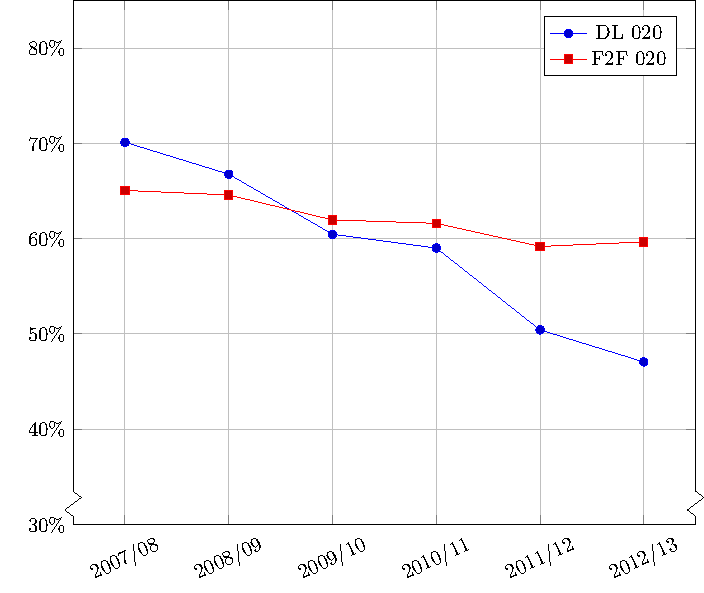
\includegraphics[width=\textwidth]{graphics/passRatesByModality020.pdf}
          % arara: pdflatex
% !arara: indent: {overwrite: yes}
\documentclass{standalone}
% Caption: Enrollment in DL
% 2007/08-2012/13

\usepackage{pgfplots}
\usepackage{pgfplotstable}
\pgfplotsset{compat=newest}

\pgfplotstableread[col sep=comma]{../data/ProcessedGradesData.csv}\enrollmentdata

\begin{document}

\begin{tikzpicture}
	\begin{axis}[
			%ybar,
			symbolic x coords={2007/08, 2008/09, 2009/10, 2010/11, 2011/12, 2012/13, NaN},
			xtick=data,
			%minor ytick={1000,2000,...,7000},
			enlarge x limits,
			scale only axis,       
			grid = both,
			ymin=0.3,ymax=0.85,
			axis y discontinuity=crunch,
			scaled ticks=false, 
			tick label style={/pgf/number format/fixed},
			legend pos=outer north east,
			restrict x to domain=0:5,
			x tick label style={rotate=15},
		]
		\addplot table[x=AY,y=020_DL_Pass_Rate]{\enrollmentdata};
		\addplot table[x=AY,y=020_F2F_Pass_Rate]{\enrollmentdata};
		\legend{DL 020, F2F 020}
	\end{axis}
\end{tikzpicture}
\end{document}

          \captionof{figure}{MTH 20}
    \end{subfigure}%
    \begin{subfigure}{.3\textwidth}
    %      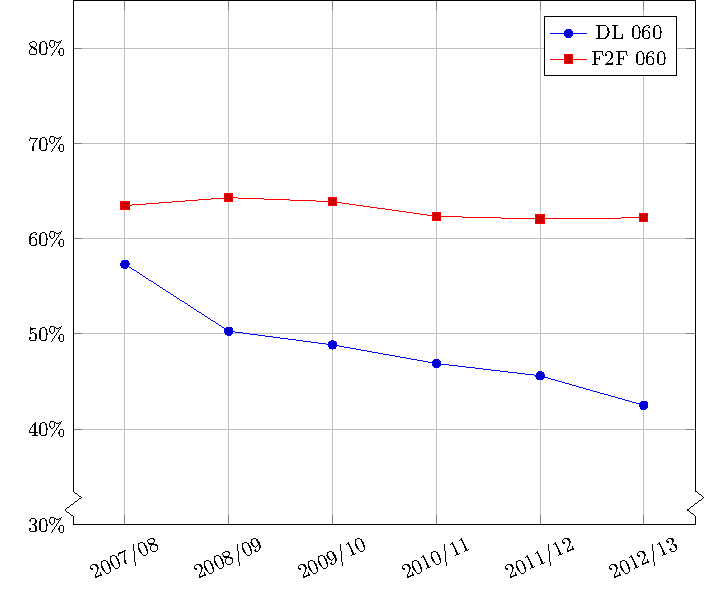
\includegraphics[width=\textwidth]{graphics/passRatesByModality060.pdf}
          % arara: pdflatex
% !arara: indent: {overwrite: yes}
\documentclass{standalone}
% Caption: Enrollment in DL
% 2007/08-2012/13

\usepackage{pgfplots}
\usepackage{pgfplotstable}
\pgfplotsset{compat=newest}

\pgfplotstableread[col sep=comma]{../data/ProcessedGradesData.csv}\enrollmentdata

\begin{document}

\begin{tikzpicture}
	\begin{axis}[
			%ybar,
			symbolic x coords={2007/08, 2008/09, 2009/10, 2010/11, 2011/12, 2012/13, NaN},
			xtick=data,
			%minor ytick={1000,2000,...,7000},
			enlarge x limits,
			scale only axis,       
			grid = both,
			ymin=0.3,ymax=0.85,
			axis y discontinuity=crunch,
			scaled ticks=false, 
			tick label style={/pgf/number format/fixed},
			legend pos=outer north east,
			restrict x to domain=0:5,
			x tick label style={rotate=15},
		]
		\addplot table[x=AY,y=060_DL_Pass_Rate]{\enrollmentdata};
		\addplot table[x=AY,y=060_F2F_Pass_Rate]{\enrollmentdata};
		\legend{DL 060, F2F 060}
	\end{axis}
\end{tikzpicture}
\end{document}

          \captionof{figure}{MTH 60}
    \end{subfigure}%
    \begin{subfigure}{.3\textwidth}
          %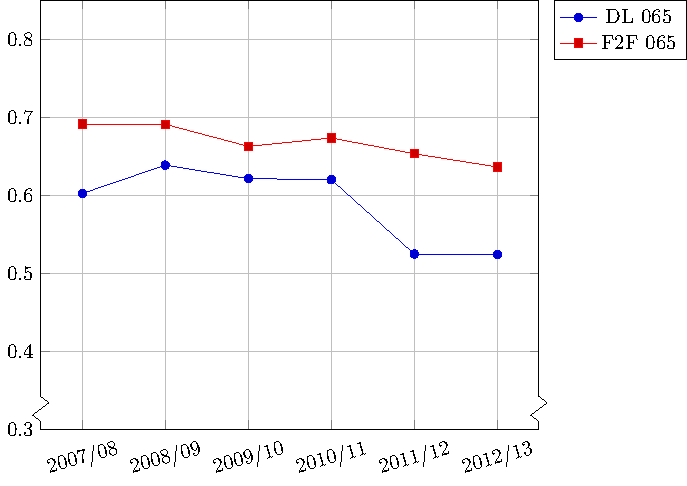
\includegraphics[width=\textwidth]{graphics/passRatesByModality065.pdf}
          % arara: pdflatex
% !arara: indent: {overwrite: yes}
\documentclass{standalone}
% Caption: Enrollment in DL
% 2007/08-2012/13

\usepackage{pgfplots}
\usepackage{pgfplotstable}
\pgfplotsset{compat=newest}


\begin{document}

% http://tex.stackexchange.com/questions/128468/problems-with-pgfplotstableread-and-relative-paths
\IfStandalone{
	\newcommand{\fromRoot}[1]{../data/#1}
	}{
	\newcommand{\fromRoot}[1]{./data/#1}
}
\pgfplotstableread[col sep=comma]{\fromRoot{ProcessedGradesData.csv}}\enrollmentdata

\begin{tikzpicture}
	\begin{axis}[
			%ybar,
			symbolic x coords={2007/08, 2008/09, 2009/10, 2010/11, 2011/12, 2012/13, NaN},
			xtick=data,
			%minor ytick={1000,2000,...,7000},
			enlarge x limits,
			%scale only axis,       
			grid = both,
			ymin=0.3,ymax=0.85,
			axis y discontinuity=crunch,
			scaled ticks=false, 
			tick label style={/pgf/number format/fixed},
			legend pos=south west,
			restrict x to domain=0:5,
			x tick label style={rotate=25},
            width=\textwidth,
		]
		\addplot table[x=AY,y=065_DL_Pass_Rate]{\enrollmentdata};
		\addplot table[x=AY,y=065_F2F_Pass_Rate]{\enrollmentdata};
		\legend{DL 065, F2F 065}
	\end{axis}
\end{tikzpicture}
\end{document}

          \captionof{figure}{MTH 65}
    \end{subfigure}

\vspace{2pc}

    \begin{subfigure}{.3\textwidth}
          %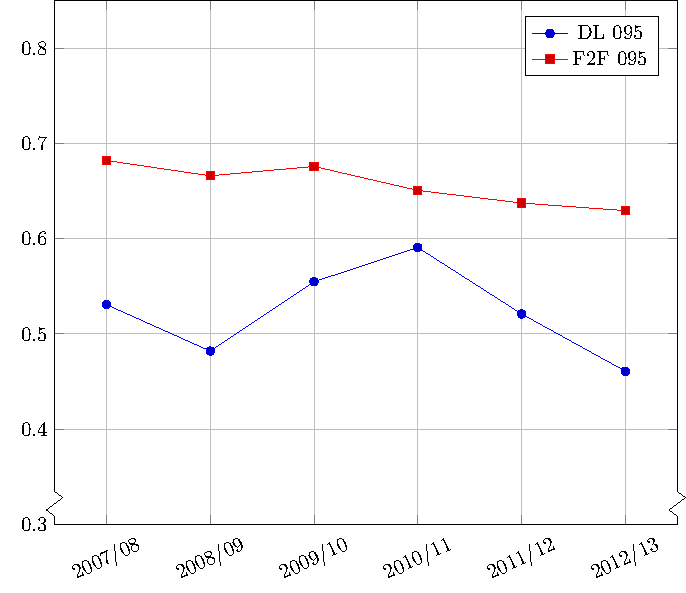
\includegraphics[width=\textwidth]{graphics/passRatesByModality095.pdf}
          % arara: pdflatex
% !arara: indent: {overwrite: yes}
\documentclass{standalone}
% Caption: Enrollment in DL
% 2007/08-2012/13

\usepackage{pgfplots}
\usepackage{pgfplotstable}
\pgfplotsset{compat=newest}


\begin{document}
% http://tex.stackexchange.com/questions/128468/problems-with-pgfplotstableread-and-relative-paths
\IfStandalone{
	\newcommand{\fromRoot}[1]{../data/#1}
	}{
	\newcommand{\fromRoot}[1]{./data/#1}
}
\pgfplotstableread[col sep=comma]{\fromRoot{ProcessedGradesData.csv}}\enrollmentdata

\begin{tikzpicture}
	\begin{axis}[
			%ybar,
			symbolic x coords={2007/08, 2008/09, 2009/10, 2010/11, 2011/12, 2012/13, NaN},
			xtick=data,
			%minor ytick={1000,2000,...,7000},
			enlarge x limits,
			%scale only axis,       
			grid = both,
			ymin=0.3,ymax=0.85,
			axis y discontinuity=crunch,
			scaled ticks=false, 
			tick label style={/pgf/number format/fixed},
			legend pos=north east,
			restrict x to domain=0:5,
			x tick label style={rotate=25},
            width=\textwidth,
		]
		\addplot table[x=AY,y=095_DL_Pass_Rate]{\enrollmentdata};
		\addplot table[x=AY,y=095_F2F_Pass_Rate]{\enrollmentdata};
		\legend{DL 095, F2F 095}
	\end{axis}
\end{tikzpicture}
\end{document}

          \captionof{figure}{MTH 95}
    \end{subfigure}%
    \begin{subfigure}{.3\textwidth}
          %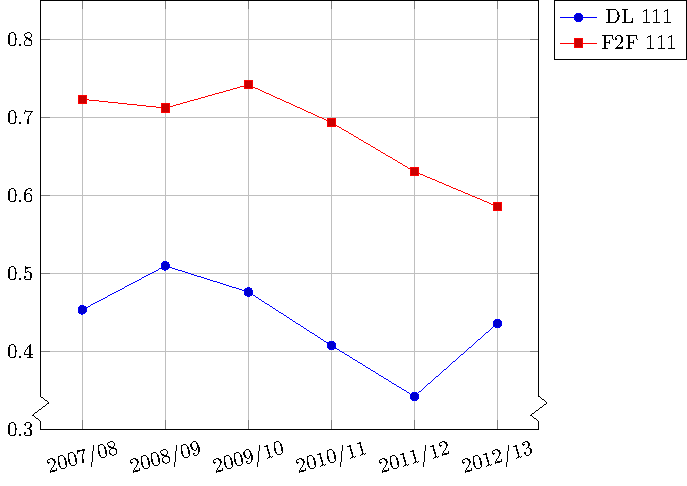
\includegraphics[width=\textwidth]{graphics/passRatesByModality111.pdf}
          % arara: pdflatex
% !arara: indent: {overwrite: yes}
\documentclass{standalone}
% Caption: Enrollment in DL
% 2007/08-2012/13

\usepackage{pgfplots}
\usepackage{pgfplotstable}
\pgfplotsset{compat=newest}

\pgfplotstableread[col sep=comma]{../data/ProcessedGradesData.csv}\enrollmentdata

\begin{document}

\begin{tikzpicture}
	\begin{axis}[
			%ybar,
			symbolic x coords={2007/08, 2008/09, 2009/10, 2010/11, 2011/12, 2012/13, NaN},
			xtick=data,
			%minor ytick={1000,2000,...,7000},
			enlarge x limits,
			scale only axis,       
			grid = both,
			ymin=0.3,ymax=0.85,
			axis y discontinuity=crunch,
			scaled ticks=false, 
			tick label style={/pgf/number format/fixed},
			legend pos=outer north east,
			restrict x to domain=0:5,
			x tick label style={rotate=15},
		]
		\addplot table[x=AY,y=111_DL_Pass_Rate]{\enrollmentdata};
		\addplot table[x=AY,y=111_F2F_Pass_Rate]{\enrollmentdata};
		\legend{DL 111, F2F 111}
	\end{axis}
\end{tikzpicture}
\end{document}

          \captionof{figure}{MTH 111}
    \end{subfigure}%
    \begin{subfigure}{.3\textwidth}
          %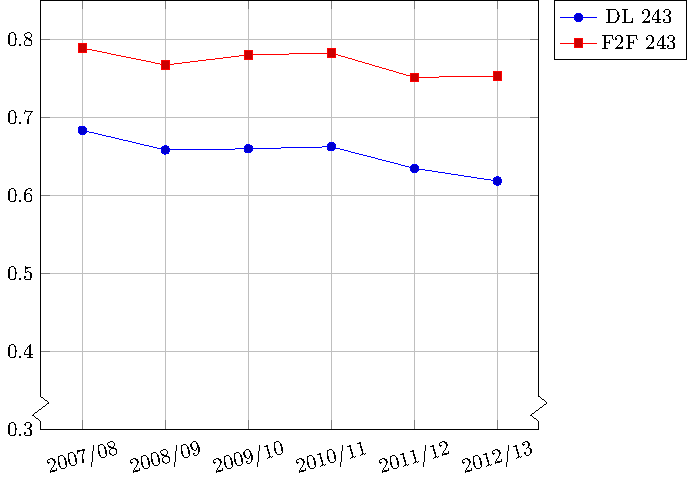
\includegraphics[width=\textwidth]{graphics/passRatesByModality243.pdf}
          % arara: pdflatex
% !arara: indent: {overwrite: yes}
\documentclass{standalone}
% Caption: Enrollment in DL
% 2007/08-2012/13

\usepackage{pgfplots}
\usepackage{pgfplotstable}
\pgfplotsset{compat=newest}

\pgfplotstableread[col sep=comma]{../data/ProcessedGradesData.csv}\enrollmentdata

\begin{document}

\begin{tikzpicture}
	\begin{axis}[
			%ybar,
			symbolic x coords={2007/08, 2008/09, 2009/10, 2010/11, 2011/12, 2012/13, NaN},
			xtick=data,
			%minor ytick={1000,2000,...,7000},
			enlarge x limits,
			scale only axis,       
			grid = both,
			ymin=0.3,ymax=0.85,
			axis y discontinuity=crunch,
			scaled ticks=false, 
			tick label style={/pgf/number format/fixed},
			legend pos=outer north east,
			restrict x to domain=0:5,
			x tick label style={rotate=15},
		]
		\addplot table[x=AY,y=243_DL_Pass_Rate]{\enrollmentdata};
		\addplot table[x=AY,y=243_F2F_Pass_Rate]{\enrollmentdata};
		\legend{DL 243, F2F 243}
	\end{axis}
\end{tikzpicture}
\end{document}

          \captionof{figure}{MTH 243}
    \end{subfigure}
    \caption{Pass Rates By Modality}\label{fig:sec3:F2FandDLpassRates}
  \end{widepage}
\end{figure}

The difference in student-success rates between on-campus courses and DL courses is an important issue for the Math SAC.  The Distance Learning Standing Committee has met to consider this issue and the factors that lead to this difference in success rates.  We can only speculate the reason for the disparity based on anecdotal evidence and professional experience.  Students may no longer see DL courses as unusual, so they may be unaware that successful DL math students should have stronger study skills, self-discipline, and time management skills than face-to-face math students absolutely need to be successful. We believe that many students register for DL math courses without adequate understanding of the study habits, time commitment, learning styles, and technical skills that are necessary for success in these classes. Anecdotal evidence suggests that some students who are aware of these issues and who would otherwise enroll in a face-to-face section still enroll in a DL section due to a lack of space in face-to-face sections.

There is currently a DL orientation available for DL students, but there is no requirement that students complete it. Furthermore, there is no information in the orientation to help students understand the particular challenges of studying \emph{mathematics} using the DL delivery methods.  In many disciplines, reading, writing, and discussion can be sufficient for learning. Students in mathematics typically do not learn best until they have also acted, by working through exercises or active problem-solving. In face-to-face classes, instructors can monitor that this learning-through-action is happening more easily. In DL courses, there is more of a need for students to rely on self-discipline to complete this portion of their learning, and this is not communicated in the existing DL orientation.


\subsection{Informing DL Students}
The Course Information Page (CIP) is accessible to students registering for DL courses and is meant to give section-specific information to students as they decide which sections to register for.   Many faculty members use this system to inform students of issues related to an online mathematics course.  For example, faculty address the misconception that a DL class requires fewer hours of attention per week than a face-to-face class. We believe that many students do not visit the CIP for DL classes and continue to be unaware of the tools they will need to be successful in a DL mathematics course.   Some faculty members send emails to registered students before the term starts, asking them to read the CIP.  It is not clear, however, how many students read this email or act on it.  The link to a CIP is only available via the online class, and not via MyPCC. This lack of redundancy may be contributing to the issue.

Other methods that are employed by DL faculty to directly communicate with their students include:
\begin{itemize}
\item using the Course Progress Notifications (CPNs);
\item placing telephone calls to students;
\item using Collaborate to hold online office hours in a kind of chat session.
\end{itemize}

\subsection{Online Homework platforms}
Faculty have sought to increase engagement by DL students through use of online homework platforms. An online homework platform can provide students with immediate feedback and also hold the student accountable for completion of assigned exercises. Faculty can monitor progress and employ formative assessment from a distance.

The SAC recognizes that program changes should come from research toward best practices.  Faculty members Wendy Fresh, Rebecca Ross, Tammy Louie, Jessica Bernards, and Diane Edwards have investigated the effects of use of an online homework system in several experiments (in both DL and F2F courses). In most cases, results from these experiments suggest there may be positive effects to using an online platform, but it remains too early to declare statistical significance. To demonstrate statistical significance in studies of this nature requires considerably large sample sizes. 

However Jessica Bernards has been able to measure one positive effect to a significant degree. Instructor Bernards taught several online sections of MTH 111, with control groups doing homework from the textbook and submitting paper write-ups, and experimental groups using online homework. The withdrawal rate was 32\% for the control group and only 16\% for the experimental group, and this difference was statistically significant ($P<1\%$).  Instructor Wendy Fresh ran a very similar experiment with online sections of MTH 60. There may still be an effect at that level, but more data is necessary to confirm with statistical significance. Both instructors noted modest improvement in exam scores among the experimental group, but again more data is being gathered to confirm with significance.

For more information on research by Instructors Bernards and Fresh for DL courses, see \vref{app:sec:onlinehwstudy}. For information on research by instructors Edwards and Louie, see \vref{app:sec:aleks} and also \cref{sec3:subset:alekspilot}. Research on the efficacy of WeBWorK (an online homework platform discussed in \ref{other:sec:webwork}) was done in \cite{focuswebwork}.  In \cite{brewer} it was found that when students are segregated by incoming ability, those who were less prepared when entering a course do benefit significantly from online homework use. As a community college, we have more underprepared students entering than universities, so this finding suggests that use of online homework may be more helpful at PCC. It is important to note that each of these studies were done with face-to-face courses; in DL courses the traditional homework alternative presents the challenge of delivery, complicating the question in favor of using online homework.

\subsection{WeBWorK}\label{other:sec:webwork}
Recent exciting developments at PCC have centered around the free and open-source online homework platform called WeBWorK that is partially funded by the National Science Foundation and maintained by the Mathematical Association of America. By spring 2014 we expect that over 20 faculty will be using WeBWorK in their courses. The math SAC is also loaning out the services of Alex Jordan to CTE and LDC science SACs to create free online homework review programs. We envision using WeBWorK for future Learning Assessment research and placement advising. We are working with Dual Credit instructors to offer WeBWorK services to Portland Public Schools.

Most of the textbooks currently in use by the Math SAC are published by Pearson Publishing, which offers MyMathLab for its online homework platform. While MyMathLab and similar commercial products come as a bundled expense with new textbook purchases, a separate online account for pairing with a used textbook purchase is rather expensive. For this reason, face-to-face instructors rarely require MyMathLab in their courses. On the other hand, Distance Learning instructors have a stronger need for an online homework platform and the majority of DL instructors do require that students use (and pay for) My MathLab.

By contrast, WeBWorK is a platform for online homework that is free and open-source. As there is no central headquarters for WeBWorK, it must be installed on a server somewhere. Since joining the Math SAC in spring of 2009, Alex Jordan has championed the implementation and use of WeBWorK at PCC. Some PCC math faculty have used WeBWorK in various capacities by borrowing server space from the University of Oregon, a relationship formed and maintained by Dr.\ Jordan. This partnership between two Oregon state institutions has been mutually beneficial. %While PCC gained server access, PCC faculty members were programming content that UO has been able to take advantage of. Each term since Fall 2011, roughly 10 sections of PCC math courses have used the UO server.

Over this period, WeBWorK users in the Math SAC lobbied Technology Solution Services to provide the Math SAC with its own WeBWorK server. While the UO server provided service to us, it came with certain restrictions and complications that prevented WeBWorK at PCC from reaching its full potential. For a time there was a chicken-and-egg situation, as TSS requested a greater usage by PCC faculty before arranging for a server while some faculty chose not to use WeBWorK because of the inconvenience of using the UO server.

In the 2012/13 academic year, faculty Chris Hughes and Scot Leavitt researched accessibility issues (in the ADA sense) alongside Disability Services. See \cite{accessibilityproject} for the full report. Among many other findings, they found that MyMathLab (at the time of the project) had many significant accessibility problems while WeBWorK was quite close to being fully ADA compliant. The open-source nature of WeBWorK meant that the few remaining obstacles to accessibility could be addressed. They recommended that the SAC cease using MyMathLab for newly developed courses and newly developed online shells. They also recommended that faculty migrate from MyMathLab to WeBWorK. Disability Services supported their recommendations, and also began lobbying TSS for a PCC WeBWorK server. Within the WeBWorK community PCC is now seen as a leader when it comes to accessibility issues. See \cite{webworkblog} for a post about this on the WeBWorK news blog. As a result of this, PCC is hosting a WeBWorK development camp in August 2014 with a central theme of addressing accessibility issues and enhancing its accessibility.

TSS partnered with the Clackamas Education Service District to deliver a WeBWorK server that will be fully implemented in winter 2014.  SAC members Alex Jordan, Chris Hughes, and Xiaolong Yao are preparing \href{http://webwork.pcc.edu}{webwork.pcc.edu} for regular use during the winter 2014 term. A backup server at \href{http://webwork-dev.pcc.edu}{webwork-dev.pcc.edu} is in place for faculty to experiment with. 

The arrival of our own WeBWorK installation has significant implications beyond homework management, particularly in the advising department. We envisage that advisors would enroll students in a `review course' that contains (mostly) pre-college practice problems, and that the student would be encouraged to sit the Compass placement test only when they are comfortable with the problems in WeBWorK. Furthermore, we can easily use WeBWorK as an advising tool to replace Hughes' Placement Advisory Test in situations when students are not happy with their placement from Compass.  The SAC should work with advising to implement this. 

\subsection{PCC WeBWorK problem library}
WeBWorK has been in use at universities for some time now, and an extensive library exists of math problems for college-level courses. However there was weak content support for basic algebra and other pre-college topics. Over summer of 2013, Alex Jordan, Chris Hughes, and Xiaolong Yao oversaw an effort to create a library of high-quality, algorithmically generated, basic algebra WeBWorK exercises which was partly funded with an IIP development grant; they received support from Kandace Kling, Debbie Neft, Jeremy Shaw, and Danielle Rice.  These exercises currently cover topics from MTH 60 and 65, and the team continues to add problems to the library for MTH 95. The library development was a success because of the strong collaboration and dedication of the three faculty members, and the foundations that Dr.\ Jordan had laid in previous years. Jordan, Hughes, and Yao presented their work at the STEM showcase (Rock Creek) in Fall 2013 (see \cref{webworkposter}). It was at this showcase that the idea was hatched to create free online homework review programs for CTE and LDC science SACs.

\begin{figure}[!htb]
	\centering
	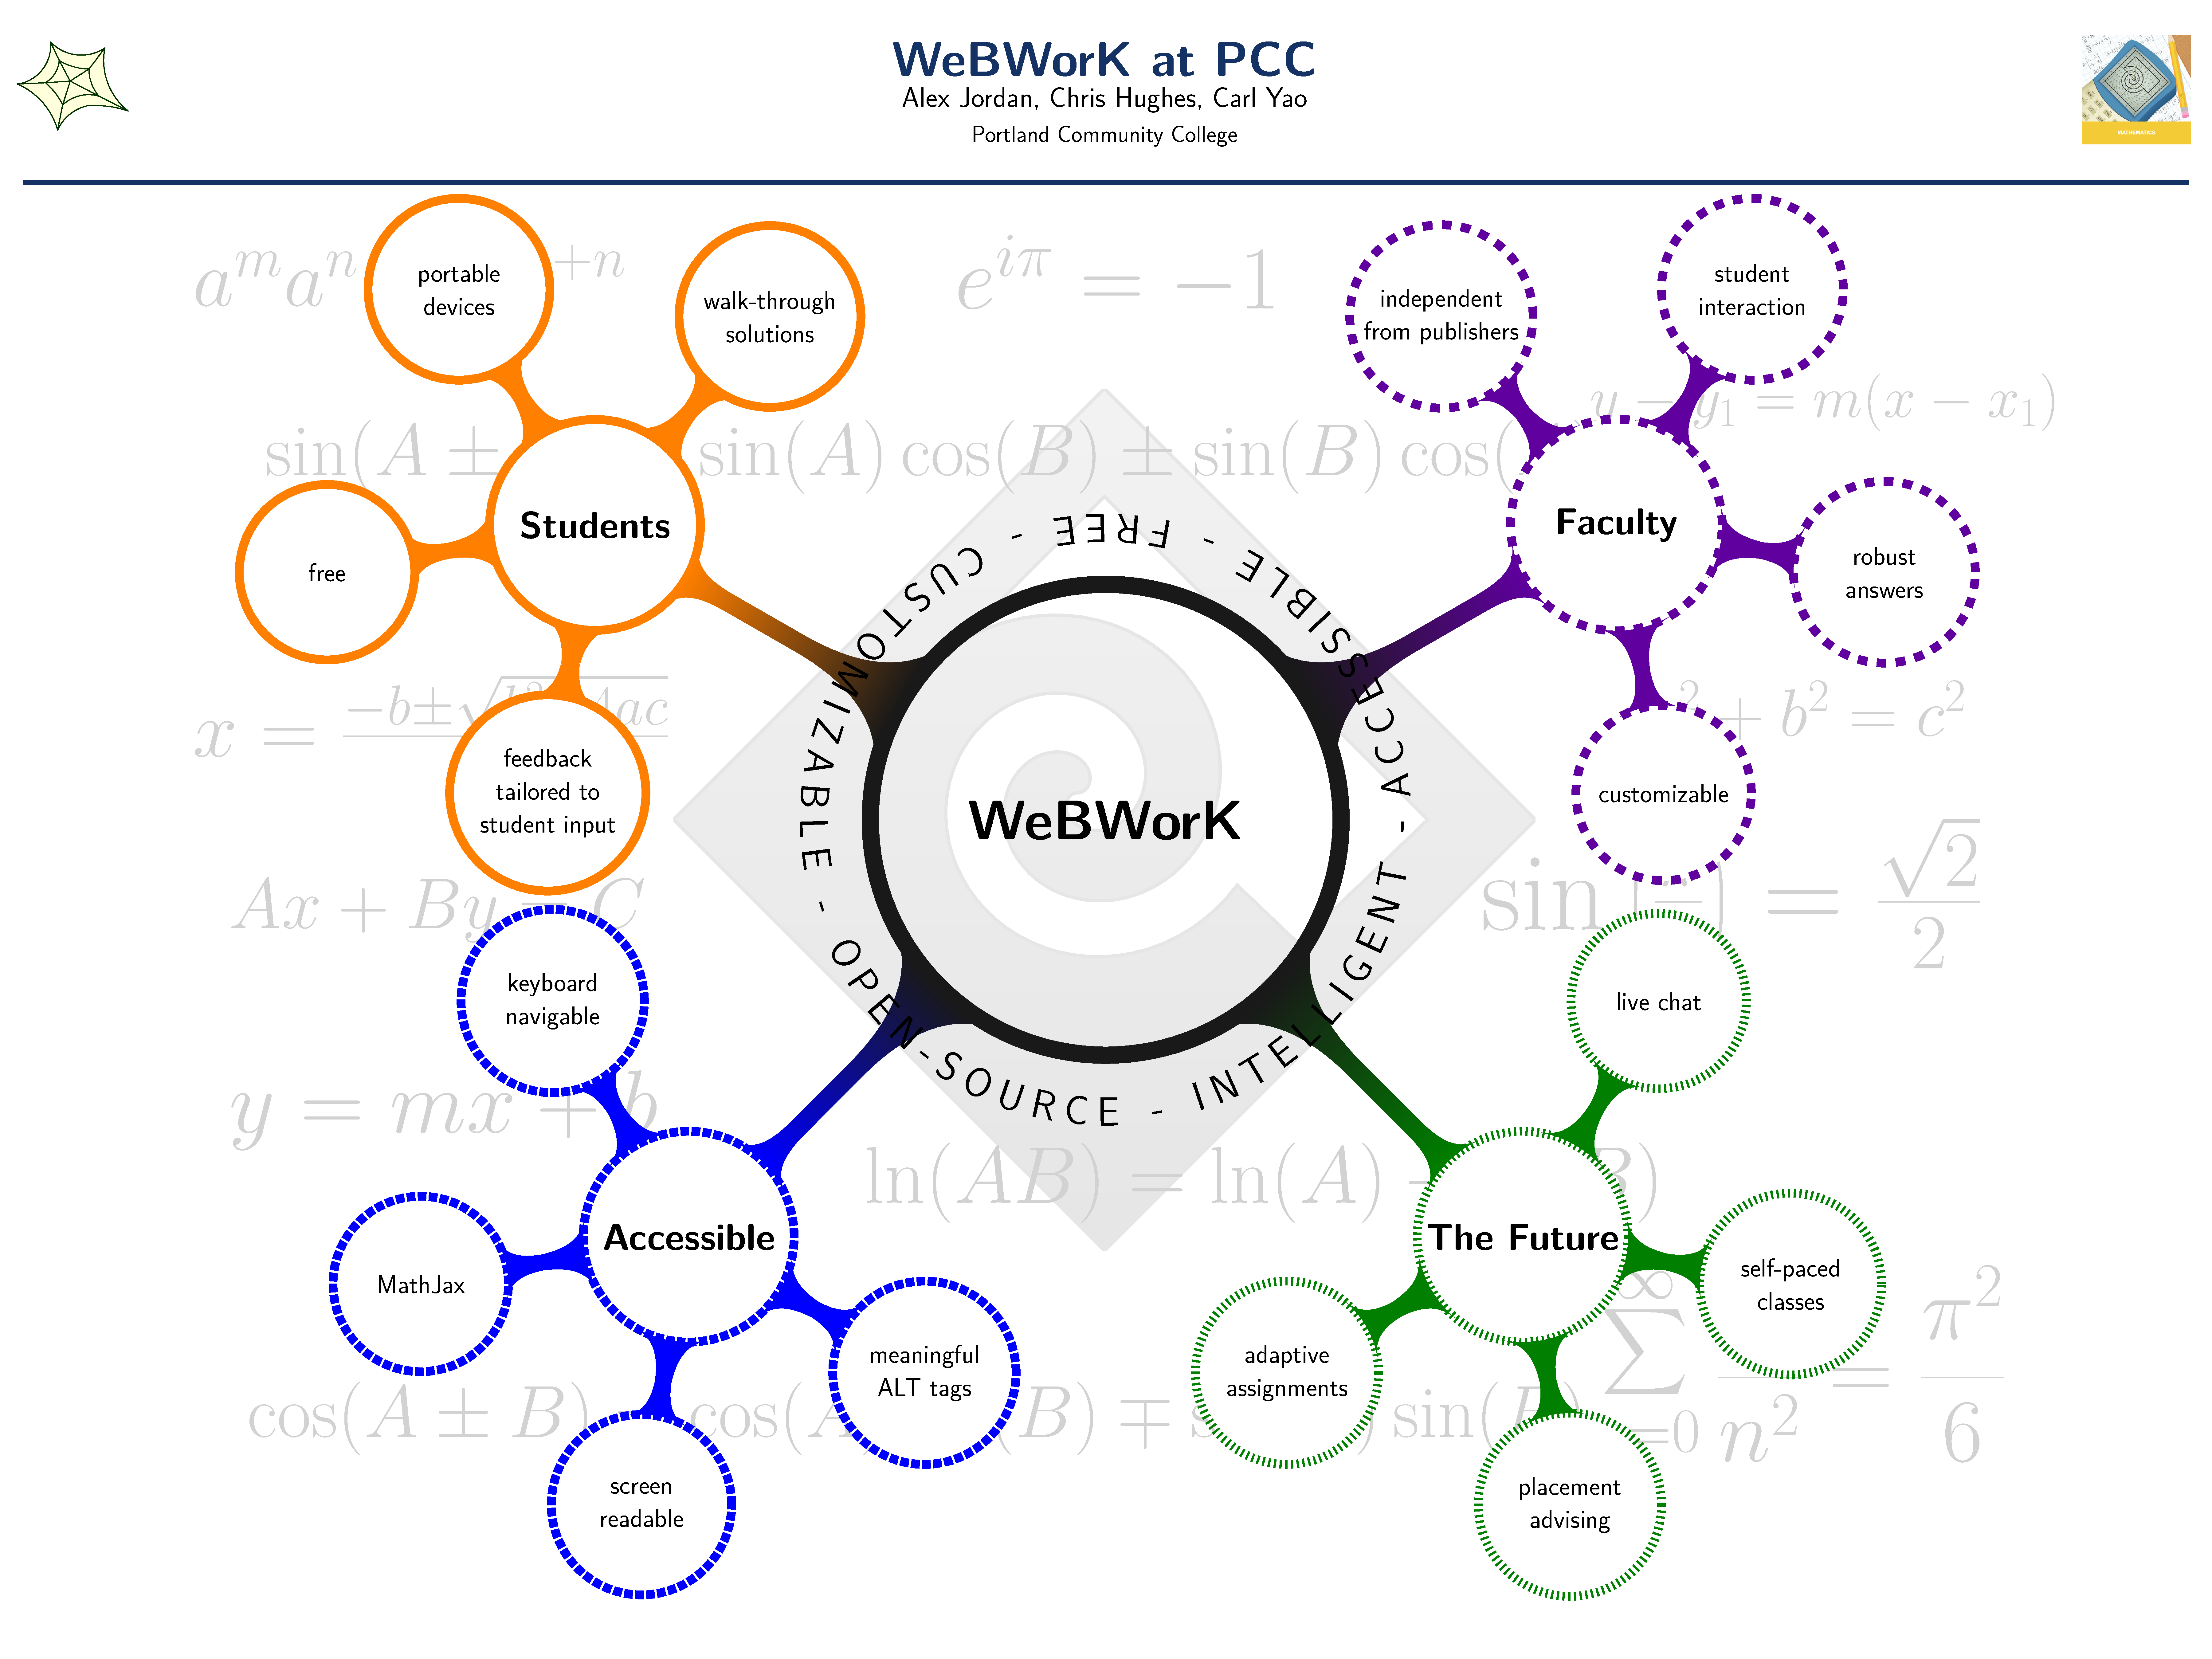
\includegraphics[width=0.5\textwidth]{webworkposter.pdf}
	\caption{WeBWorK poster from the PCC STEM Showcase}\label{webworkposter}
\end{figure}

As time and funding progress, SAC members with the requisite coding experience hope to add more problems to this PCC library, expanding into the arenas of MTH courses 20, 111, 112, 243, and 244. It is important to note the level of quality of the problems from this library. Each problem has a full walk-through solution coded along side the question which can be put to use by faculty in a number of ways. Each problem is given fine attention to detail so that automated feedback messages to the students are as informative as modern technology can allow. This high level of quality requires time and experience to achieve. However it is necessary if any instructor hopes to use WeBWorK as a teaching tool and not just an assessment tool.

\subsection{Concerns about DL offerings}
Each of the following three issues have been raised by SAC members, and during the 2012/13 academic year a group of concerned faculty met to discuss them. The meetings were informal and no binding decisions were reached.
\begin{itemize}
\item Faculty are concerned about whether or not Distance Learning is an effective way to deliver math content, especially in light of the low pass rate statistics seen in \cref{fig:sec3:F2FandDLpassRates}. Successfully learning mathematics generally requires heavy active engagement. Face-to-face courses facilitate this engagement by requiring students to be in the physical presence of their instructor and fellow students. In DL courses, the imperative to remain engaged must come mostly from the student's own sense of responsibility and interest.
\item Faculty are concerned about the quality and consistency of current DL courses. Some faculty rely on publisher content such as electronic versions of textbooks, while other faculty have created complete sets of online notes themselves and use e-books only as secondary resources. Instructor Chris Hughes serves as an advisor to online faculty creating new courses, and makes recommendations to improve course quality and observe accessibility standards. However there is no enforcement of the online advisor's recommendations.
\item Faculty are concerned about the portion of a student's grade that may be computed from online homework. Compared to traditional homework, online homework is more readily vulnerable to cheating. With many math exercises, the exercise can literally be typed in to Google and the search engine itself provides an answer. Online homework provides fewer obstacles for a dishonest student to employ someone else to do their homework for them. In fact, in Craigslist sites nationwide, all one need do is search for `mymathlab' to find advertisements from those who will `take your online math course for you' at a cost. The math SAC has always wanted its online courses to mirror its face-to-face courses, and as a consequence has never created CCOGs that treat face-to-face and online courses differently. This has made it difficult to place any cap on the portion of a grade that may be computed from online homework. There is also no consensus on what an appropriate cap would be.
\end{itemize}

\subsection{Recommendations}
Our main recommendations concern how to best inform students about the particular skills that a distance learning student should have or adopt in order to be successful. We also recommend enacting some prerequisite items for DL registration to help give these skills to students. Lastly there are some recommendations that do not fit these descriptions. Many of these recommendations hold for F2F courses as well, and may be repeated elsewhere in this program review. 
\begin{description}
\item For the Math SAC
\begin{itemize}
\item Collaborate with advising to implement a WeBWorK-based review mechanism for would-be placement test-takers.
\item Consider how the quality of online courses could be regulated more. 
\end{itemize}
\item For Administration/Advising
\begin{itemize}
\item Collaborate with the Math SAC to implement a WeBWorK-based review mechanism for would-be placement test-takers.
\item Give students more information on DL responsibilities and make students aware of the difference in student-success statistics between DL and face to face courses.
\item Encourage students to contemplate why they seek to take a DL course and reflect upon whether it will be aligned well with their learning style and personal skill sets.
\end{itemize}
\item For Administration/DL/TSS
\begin{itemize}
\item Have the online orientation linked from the registration tool in MyPCC and require that students complete this orientation before registering for a DL class.
\item Include a section in the DL orientation that addresses the specific challenges that DL brings to mathematics courses. Perhaps only students seeking to register for a mathematics DL course would be required to complete this section.
\item Add redundant access to the Course Information Page. Along with access through the online Class Schedule, the CIP could be available through MyPCC on the home page for a course and through Desire To Learn.
\item Include a pop-up or hover-over window that is activated when a student tries to register for a DL MTH class that gives specific information about the challenges of DL Math courses.  
\end{itemize}
\item For Administration/Other
\begin{itemize}
\item Require students to demonstrate pre-requisite computer literacy skills such as those taught in basic internet skills (CAS 104), beginning Word (CAS 216), beginning keyboard (CAS 121), and basic computer skills/MS Office (CAS 133).
\item Develop and require a basic DL/computer skills competency course, possibly offered during week 0 of the term.  
\item Provide opportunity for faculty professional development in research design and data analysis to help with research efforts on the efficacy of online homework.
\item Provide support for further development of WeBWorK related projects, including a larger library of math problems for courses beyond 60/65/95, enhancements of the WeBWorK engine, and content for placement advising/review.
\end{itemize}
\end{description}

\section[Curricular changes resulting from educational initiatives]{Has the SAC made any curricular changes as a result of exploring/adopting educational initiatives (e.g., Service Learning, Internationalization of the Curriculum, Inquiry-Based Learning, Honors, etc.)?  If so, please describe.}


\subsection{Math 111H College Algebra: Honors}

The course has been offered only at Sylvania campus -- Winter 2012 (12 students), Winter 2013 (22 students), Spring 2013 (15 students), and Fall 2013 (17 students).  Ronda Lively was the instructor the first three terms, which allowed her to evolve her materials and activities.  Ann Cary is teaching the Fall 2013 term, and has collaborated closely with Ronda Lively. 

The honors course must cover all of the same material as the regular course. It is stressed that honors versions of a course should not be ``harder'', but different in the use of class time and activities/assignments.  There should also be a component of Community and Environmental Responsibility, which is a PCC core outcome that is usually difficult to place in math courses.  Instructor Lively regularly teaches MTH 111 and MTH 111H during the same term.  The same exams are given in both courses.  There were differences in the other evaluation criteria used in the courses.  In the MTH 111 class, students submitted take home graded worksheets and participated in an in-class graded group activity.  The evaluation of the students in the MTH 111H class included:
\begin{itemize}
\item a collaborative computer project involving math history and investigation of several applications of math
\item a team quiz-grading activity where each group wrote a key and grading rubric, then applied it to two (fictional) students' quizzes
\item a community tutoring project:  over several weeks, they found someone to tutor in math (friend, neighbor, family member, \ldots) and then wrote a paper on their experience
\end{itemize}
Since the overall student ability level was high, there was time in class to investigate other topics of interest related to college algebra.  Each term there were several students enrolled that signed up because of the time slot, not because they were strong in math.  An encouraging development was that the stronger students took the less prepared students under their wings and helped those few struggling students be successful.


\subsection{Social Justice Workgroup}
A Math and Social Justice workgroup was formed by Ann Cary and Emiliano Vega in response to a national convention they attended. The group has collected and disseminated data sets and activities to participating instructors and has gained interest and participants from other disciplines at PCC as well as area high school math instructors and community activists in Portland. More importantly, the group has the focus of providing a forum on how to discuss potentially sensitive subjects in a classroom setting when using application problems and how to be more culturally and socially aware of individual students and classes. The information they gathered has been brought to participating instructors and has improved the pool of activities and application problems available, improved the ability of instructors to work effectively with the broad demographic of students and co-workers, and also continues the college's focus on two Core Outcomes: Community and Environmental Responsibility and Cultural Awareness. For a sample of material from this workgroup, see \cref{app:sec:socialJustic}.

\subsection{Service Learning}
Service Learning has been a part of many math instructors' courses at PCC, but has been deepened and new supports exist through the Service Learning website. The Service Learning website includes additional resources and syllabi submitted by participating Instructors at PCC. In addition, Service Learning will been added to some CCOGs evaluation criteria to encourage instructors to incorporate Service Learning in their math classes. In addition, Jeff Pettit participated as an observer in the Service Learning training cohort at Sylvania campus, connecting with instructors in other disciplines and understanding how Service Learning is employed in other courses. This has led to new curriculum in his Statistics courses and upper-division courses where Service Learning was not originally employed.

\subsection{Developmental Education Math Study Group}
A new committee was formed by the SAC to address developmental math completion rates. The committee is researching the feasibility, cost and difficulty associated with implementing ``pathways'' beyond the current calculus focused MTH60-95 courses. The committee is considering options for employing career-based math course series and a statistics-based math course series.

\subsection{Placement Test Reform Group}
In addition, a committee is being formed to address placement test reform. The group intends to better measure students' needs beyond the current math-skills Compass test. We hope to find a way to measure key traits and needs of students to connect student populations with the support needed to better guarantee success.

\section[Present dual credit relationships]{Are there any courses in the program that are offered as Dual Credit at area High Schools?  If so, describe how does the SAC develops and maintains relationships with the HS faculty in support of quality instruction. Please note any best practices you have found, or ideas about how to strengthen this interaction.  }

During the 2012/13 academic year, PCC dual credit for mathematics was awarded for seven mathematics courses.  Classes were offered at seven high schools and there were a total of twelve instructors certified to teach PCC dual credit mathematics classes.  There were a total of 750 unduplicated students who enrolled in at least one PCC dual credit mathematics class and collectively those students earned 6032 mathematics credits through PCC.
In the fall term of 2012, an ad hoc committee was formed in the mathematics SAC to investigate the status of our dual credit program.  The formation of this committee was prompted, in part, by the discovery that several of the posted dual credit syllabi described courses that bore little resemblance to the course for which students were earning PCC credit.  The committee decided that the root cause of this disconnect was a lack of robust support on our part.  Three concrete actions were taken to address the disconnect:
\begin{itemize}
\item Each dual credit mathematics instructor was assigned a team of two support faculty from the mathematics departments at PCC.  Each pair of support faculty visited their assigned instructor at that instructor's high school.  These meetings were rather informal; the intent being to establish a concrete support team for each high school instructor.
\item A two-day mandatory summer workshop was organized by the committee in conjunction with Beth Molenkamp; at that time Beth was the coordinator of PCC's dual credit program.  At the workshop each dual credit instructor was tasked to complete a robust (and accurate) syllabus for each of their dual credit classes.  The PCC faculty helped with this task and all of the dual credit instructors now have syllabi that truly reflect the nature of the course for which the students are earning PCC credit.  The remainder of the workshop was spent sharing resources and pedagogical tactics used by various PCC faculty in the courses for which dual credit is also offered.
\item A Google Drive site was created to share resources.  Although the inspiration for this site was to give our dual credit faculty easy access to shared resources, the pooling of resources is obviously of great benefit for PCC faculty as well.
\end{itemize}

\section[Future dual credit relationships]{Does the SAC plan to develop any additional Dual Credit agreements with area high schools?  If so please describe.   If not, what does the SAC see as barriers to developing further dual credit agreements. }
Students at Central Catholic High School will get their first opportunity to earn PCC mathematics dual credit during the 2013/14 academic year.  This adoption was coordinated through the dual credit program; that is, the math SAC played no active role in the creation of this dual credit agreement.
There is concern in the mathematics SAC that the state's 40-40-20 initiative, and the accompanying bills aimed at encouraging high school students to earn college credits, might lead to a dramatic increase in the number of high schools offering dual credit for mathematics courses.  What's most worrisome about this is that there are not that many high school mathematics instructors who meet PCC's qualifications to teach post-100 level mathematics courses.  We are concerned that the day might come where we are pressured to lower those standards or, of even more concern, we are pressured to start awarding PCC dual credit for developmental mathematics courses (MTH 95 or below).


\section[Other significant curricular changes]{Identify and explain any other significant curricular changes that have been made since the last review.}\label{cur:sec:other}

\subsection{MTH 20 moved to the Math SAC from the DE SAC}
The MTH 20 curriculum was moved into the Math SAC from the DE SAC in Fall 2012, bringing all math curriculum under the same SAC.  This move was meant to help create consistency in the CCOGs across the spectrum of math courses, as well as ensure that the MTH 20 curriculum is adequately preparing students for the next math course.

Sylvania Campus, which had a separate DE Math department altogether, transitioned its DE Math instructors into the Math Department in Fall 2013.  A Math Integration Work Group was formed and charged with creating a seamless path for this transition.  With the DE Math instructors in the Math SAC and the current move toward success in pre-college math courses, the Math SAC?s focus is on producing high-yield instructional practices, student success, and completion across the span of math courses offered by the college.
 
\subsection{MTH 20 Proposed Credit Change: 4- to 5-credits}
MTH 20 (Basic Math) is a content-heavy course that covers topics such as fractions, decimals, signed number operations, geometry, proportions, and percents.  It can be argued that the amount of material covered in MTH 20 is greater than in any of our other mathematics courses.  At times, instructors are forced to either minimize required topics or occasionally cut them entirely due to time constraints.  Because of this, for years many MTH 20 instructors have wanted to increase the number of credits for the course.  

In October 2012, the SAC received a memo from the DOIs related to class sizes in which we were encouraged to consider converting MTH 20 from 4- to 5-credits.  At that point a subcommittee was formed by the SAC to investigate the benefits and consequences of increasing the number of credits on the course.  The committee looked into the financial aid impact on students, the impact on degree/certificate programs, and the impact on classroom availability.  It also rewrote the CCOG to include study skills and increase the emphasis on reading graphs and geometry in the course.  

In April 2013, the Mathematics SAC approved the conversion of MTH 20 from a 4-credit course to a 5-credit course.  The conversion was then approved by the Curriculum Committee in November 2013.  Unfortunately, the current DOIs denied the recommendation in late November.  Since the original recommendation came to the Math SAC in 2012, the DOIs have changed and it seems that the new DOIs perspectives and wants for the math curriculum are different.  The Math SAC may, however, have another opportunity to readjust the content-heavy course while reorganizing DE math in the next few years. 

\subsection{MTH 60/65/70/95 Curriculum Alignment}
The Math SAC recognized that students successfully completing MTH 65 often had difficulty passing MTH 95.  The same was true for students transitioning between MTH 95 and MTH 111.

It was thought that creating more continuity between the MTH 60/65 series and MTH 95 would improve student success.  To this end, during 2008/09, a committee was created to redesign the 60/65/95 curriculum with an eye toward carefully preparing students for the rigor of college level mathematics.  While MTH 60, MTH 65 and MTH 95 had been traditionally taught as algebraically focused classes, the committee adjusted the curriculum to reflect the need for students to be able to understand mathematical information via the ?rule of four;? algebraically, graphically, numerically and verbally.  This was done to prepare students for the demands of college level math and to align with the best practices of our field.  Importance was also placed on the use of a graphing calculator in MTH 95 to aid in this.  These changes were also reflected in the intermediary course in the MTH 60/65/95 series: MTH 70.
 
As with all curricular changes, there continues to be a need for ensuring that all of the instructors receive the necessary communication and support in implementing these changes.  This is especially true for the part-time instructors who are teaching a large portion of the MTH 60-95 courses.  However, with the nature of the part-time instructor?s working conditions, this continues to be a challenge.  The Math SAC requests more support from the administration to provide the necessary funding for part-time instructors to attend course-specific meetings similar to that held for MTH 95 instructors at the Sylvania Campus prior to the Fall 2013 term.
 
\subsection{Replaced MTH 111A/111B/111C with MTH 105 and MTH 111}
In 1997 the Math SAC split MTH 111 into three courses in order to target different student populations: MTH 111A for liberal art students, MTH 111B for business and other non-technical majors, and MTH 111C for Science and Engineering.  In our last Program Review (Fall 2003?2008), it was mentioned that we eliminated MTH 111A and resurrected MTH 105.  Since the last Program Review, MTH 111B and 111C have merged again into MTH 111.  Since 1997 when MTH 111 was split into three distinct courses, the CCOGs for MTH 111B and MTH 111C had grown more and more similar since both courses were prerequisites for the same courses (MTH 243 and MTH 251) so they needed to cover the same content.  MTH 111B had a reputation for being an easier course and many instructors noticed that students in MTH 112 who had taken MTH 111B instead of MTH 111C were less prepared.  Since the two courses no longer served different purposes, and since having two courses serve the same purpose was creating problems with student preparation for subsequent courses, we decided to unify MTH 111B and MTH 111C into a single college algebra course: MTH 111.
 
\subsection{MTH 243 Credit Change: 4- to 5-credits}
The Math SAC increased credits for MTH 243 (Statistics I) from 4-credits to 5-credits for several reasons, most of which were related to a need to increase the contact hours from four hours to five hours.  In order to address the needs of future coursework in statistics as well as sufficient coverage of material for transfer to many universities, it was essential to add more material to the 4-credit MTH 243 course.  Increasing the credit hours allowed for the necessary contact time to cover such material appropriately.
 
 
Five contact hours allows for more integration of technology into the classroom, since these technology skills are best learned in the classroom. Formerly, it was often difficult to have meaningful technology-oriented statistical classroom exercises due to the lack of classroom time.
 
The change to five contact hours also gives sufficient time to fully engage the students with critical thinking exercises and quantitative and statistical literacy discussions.

\subsection[Creation of AMP/MTH008]{Creation of Two Accelerated Review Courses (referred to as the Accelerated Math Program, or AMP) MTH 07 and MTH 08}
 
\begin{description}
\item[MTH 07: Accelerated Basic Math Review]  This course presents a review of basic math skills and provides the opportunity for guided practice.  Topics include operations with whole numbers, fractions, decimals, proportions and percents.

\item[MTH 08: Accelerated Introductory Algebra Review] This course presents a brief review of basic algebra skills and provides the opportunity for guided practice.  Topics include real number operations, manipulating linear expressions, solving linear equations, and graphing linear equations in two variables.
\end{description}

These two courses were designed to meet the needs of the following two student populations:
\begin{itemize}
\item students who have previously learned the material and are able to move on the next class with a brief amount of review, and
\item students who have difficulty with the material and can work on a variety of the regular course material in advance of taking the regular course.
\end{itemize}

Both courses are offered for one week in-between terms and are 15 non-credit lab hours.  They are taught with a combination of mini lectures and computer practice/instruction.  At the completion of each course, students retake the Compass placement test.  Each term a significant number of students taking these courses have placed into a MTH course above their previous Compass placement.

Sections have been offered at the Rock Creek, Southeast, and Cascade Campuses, with most offerings at the Cascade Campus.  Data from the sections taught at Cascade Campus since 2010 can be viewed in \vref{app:sec:ampdata}.
 
\subsection{Clarified CCOGs Requirements and CCOG Addendums}
It was found that there were numerous discrepancies among different sections of the same course having different instructors regarding the material being presented. In an effort to ensure that students completing different sections of the same course had similar mathematical competencies, the SAC determined that communicating the requirements for a course needed to be made more concise.  Also, since the curriculum had significantly changed, we wanted instructors who had previously taught the course to know about these changes.  The CCOG for each course was intentionally written more clearly and now includes specific minimum requirements for testing and grading.  In addition, each CCOG now has an addendum that clearly shows examples of what is expected in terms of content, mathematical notation and presentation as well as well defined assessment strategies.  This practice has now been adopted for most of our CCOGs.
 
\subsection{Elimination of MTH 91 and MTH 92}
MTH 91 and MTH 92 were created to address the issue of the high failure rate in MTH 95 by splitting up the content of MTH 95 into two terms.  The course sequence was discontinued after data showed that students taking MTH 91 and 92 were not successful in the subsequent course MTH 111. It was found that after taking these slower paced classes, the students were not prepared for the speed of the MTH 111 course.
 
\subsection{Changes in MTH 251-254}
The calculus series has been more strongly split into Calculus I/II and Calculus III/IV by requesting the publisher split the current text into two sections. This change altered the need for Maple in MTH 251 and MTH 252.  Maple is an expensive graphing software package that students buy for one year but generally use only for Calculus IV. Attaching Maple to the new second half of the book solved the issue of students losing access to it if they took more than one year to complete the Calculus series.

\subsection{Math Study Skills Material Development}
Research has shown that students with strong study skills are more successful in their academic pursuits than their counterparts.  A common characteristic of students entering developmental mathematics courses involve poor study skills.  In an effort to help students build a stronger awareness of how a successful student studies, math SAC member Jessica Bernards from the Rock Creek Campus created a Math Study Skills program to be used in our developmental math courses.  This program consists of seven topics all relating to study skills specific to mathematics: how learning math is different, resources available for help at PCC, time management, listening and note-taking skills, how to do homework, test taking strategies, and overcoming math and test anxiety.  Each lesson is broken up into three parts: a short video to be watched by students outside of class, a student worksheet to be completed in conjunction with the video, and an in-class discussion lead by the instructor. Additionally, each topic has quotes from successful students which help strengthen the ideas in each video.  Many math instructors across all campuses piloted the program in the Spring 2013 and are continuing to use it this Fall 2013. For winter 2014, fourteen DE math instructors have reported that they will be using it. The study skills website can be found at \cite{studyskills}.
 
\subsection{MTH 111/112 Document Project}\label{cur:sec:111/112doc}
In Winter 2010, Math SAC member Chris Hughes proposed that the SAC write its own MTH 111/112 textbook. This idea sprung from a general frustration with commercially available textbooks for this sequence.  Available books tend to fall on one end or another of a spectrum ranging from template-based and lacking in conceptual understanding to abstract and lacking in guidance for students.  We seek something with better balance.  Since then, other motivations for such a project have arisen, including the high impact it would have on student pocketbooks.

Initially over 10 members of the Math SAC became involved, submitting ideas and small sections of what might someday become a textbook.  As time passed, four SAC members (Chris Hughes, Alex Jordan, Ann Cary, and Steve Simonds) maintained serious interest in the project.  Piecing together earlier work from the larger group, expanding on that work, and editing, these four produced a rough draft chapter representing about 10\% of a final product. (Given that this draft would need editing, we estimate that represents 5\% of the work necessary for completion.)

As of Spring 2013 roughly 10\% of a finished product had been produced.  At this point the four remaining editors put active work on hold until some level of release time can be secured that would enable completion in a timely manner.  A completed textbook for the entire sequence could be drafted with three faculty taking one-third release time for two consecutive terms.  An additional such term would provide for peripherals such as guided lecture notes, an online homework library, and LiveScribe videos. The progress to date can be found at \cite{mth111project}.
 
\subsection{Supplemental Course Packets}
Textbooks that the Math SAC selects for courses occasionally have gaps when compared to the CCOGs for that course.  Supplemental course packets were created to fill in the gaps and are required for those specific classes.  These include explanations of topics not covered in the textbook at all as well as example problems to fully cover a topic that might be lacking in the textbook examples.  Supplemental course packets have been created for MTH 60, 65, 95, 111 and 112, and these can be freely downloaded from the Math department's web site \cite{pccmathdept}.
 
\subsection{MTH 251 Lab Manual}
Since the late 1990s, MTH 251 has been taught in a lecture/lab format.  From that time through the late 2000s the materials used during the lab portion of the course were modified on a frequent basis.  By 2009 the lab manual had devolved into a collection of random problems.  The problems themselves were fine, there was simply no connection between one set of problems and the next.  There also were limited central themes to any one set of problems.

In the summer of 2009 faculty member Steve Simonds rewrote the lab manual from scratch.  The problem sets were written in a deliberate way to help students develop deep understanding of key concepts covered in the course.  The majority of the problems from the prior lab manual were then shuttled to the appendix as practice problems for outside of class.  All of the practice problems were fully keyed so that the students could continue thinking about the ideas (and practicing the skills) covered in lab and then determine for themselves if they have come to reasonable conclusions.

\subsection{MTH 105 Course Material Flexibility}
Each math course has traditionally used the same SAC approved textbook district-wide.  The Math SAC broke from this tradition and voted to allow MTH 105 instructors to choose their own course material, provided it meets the approval of the MTH 105 CCOG.  Unlike other math classes, MTH 105 is not a prerequisite for other math courses, and is a terminating math course for many of our students.  Each term, the instructor selects three to five topics from a list of 17.  This allows the instructors flexibility to teach material appropriate for the student population of each class.

\subsection{Alternative Learning Center (ALC)}
The ALC classes are self-paced pre-college math classes\footnote{The Alternative Learning Center was the previous name for the current Student Learning Center.}  They are designed for students to work independently at their own pace and allow them to focus on specific topics.  Consequently, a wide range of students take these classes: students who are afraid to take a math class and want to get back into math slowly; students who failed a class once or several times; students who feel that they placed too low on the placement test and just need a review; students who want to get through the material quickly; and international students who know the math but not the English terminology for it.  At Sylvania, the majority of students who take ALC are students who have failed math classes, sometimes many times.

Historically, the ALC math classes have been offered at Sylvania Campus, housed by the Developmental Education SAC, and covered math content up through MTH 65.  Since Summer 2012, they have also been offered at Southeast Campus.  Since Winter 2013, ALC is housed in the Math SAC and, since Fall 2013, it also includes MTH 95. For a more thorough look at these changes, see \vref{app:sec:alc}. Considerations are currently being made to find ways to have ALC Math also at Cascade and Rock Creek.  Students from these campuses are already using ALC Math at Sylvania and Southeast and are undergoing the hardship of travel just so they can take these classes.

Enrollments at Sylvania and Southeast both show that there is clearly a need for these classes.  Research done by PCC?s Institutional Effectiveness on data from five years at Sylvania shows that students who complete ALC classes successfully pass their classes at a higher rate than before taking ALC classes.  (See \vref{app:sec:effectivenessALC}.)  It would therefore be well worth looking into using the ALC classes as an early intervention when students fail math classes.  At Sylvania, for instance, it has become more and more of a practice that some full-time advisors have made themselves very familiar with these classes and suggest them to students early on.  Others send them to the Math Coordinator for further advising regarding the math classes.
 
\subsection{MTH 84 - Introduction to \LaTeX}
In Spring 2010, Math SAC members Alex Jordan and Chris Hughes proposed a pilot course to teach the typesetting software \LaTeX\footnote{used to typeset this outstandingly well-made document}.  The experimental course was piloted for three consecutive terms (Fall 2010, Winter 2011, and Spring 2011) and then adopted by the SAC as MTH 84.  The course was first run (as MTH 84) in Winter 2012, and has run each term since with one section per term. MTH 84 is a one credit pass/no-pass course. Its modality has been DL, although the CCOG does not prevent a face-to-face version.  The course serves students in many areas.  \LaTeX\ is a useful tool in math, the sciences, in graphic design, and in publishing. 
 
\subsection{MTH 76 SAC Approval}
The SAC approved the CCOG for an introduction to GeoGebra course. The course is planned to run as a pilot for Spring 2014 and Summer 2014 with tentative approval to let it run as a permanent course Fall 2014.  The audience for the course includes PCC students, PCC instructors who wish to use it as a teaching tool, and K-12 teachers who wish to use it as a teaching tool.  The course was requested by high school teachers participating in the Dual Credit workshop in the summer of 2013.

\subsection[ALEKS pilot]{Pilot using ALEKS Technology in Two Math Courses during 2012-2013 AY}\label{sec3:subset:alekspilot}
ALEKS technology requires students to complete each mathematics topic successfully, keeps track of student work time, provides instant feedback, routinely assesses students and requires them to revisit previously learned material.  It allows students to study a variety of topics at a time and minimizes practice of mastered material. Two pilots of ALEKS in MTH 20 and MTH 112 were conducted.

\begin{description}
\item[MTH 20: Basic Mathematics] ALEKS was incorporated into six online and six on-campus MTH 20 classes.  Data was compared to the previous year?s MTH 20 classes taught by the same two instructors, Diane Edwards and Marilyn Marshall.  On average, courses using ALEKS had noticeably higher pass rates than non-ALEKS courses.  For example, there was an 11\% increase in pass rates in on-campus ALEKS classes fall term 2012 compared to non-ALEKS fall term 2011 classes.  Both on-campus and DL classes showed increased passing rates using ALEKS.  In addition, a few students each term were able to complete two courses during one term, finishing Basic Mathematics early and then successfully completing MTH 60.

\item[MTH 112: Elementary Functions] ALEKS was incorporated into one Elementary Functions section and compared with two traditional sections, all taught by faculty member Tammy Louie.  In this small sample, both the grade distribution and pass rates were similar.  However the student retention rate in the ALEKS class was 17.3\% higher than in the non-ALEKS classes.  
 
 \end{description}
 
In both pilots students were observed to enjoy using ALEKS and increase their study time while using ALEKS.  More detailed data can be found in the \vref{app:sec:aleks} concerning both pilot projects. These pilots of ALEKS had noticeable success with data and student perception and involvement.  Further exploration of ALEKS technology should be pursued as a possible option to improving student success in mathematics courses.
 
\subsection{MTH 112 Formula Sheet}
The SAC approved a standardized ``formula sheet'' for use in MTH 112.  Math SAC member Wendy Fresh revised and submitted a formula sheet edited from one provided by SAC member Pete Haberman.  The page was added to the course CCOGs to help guide instructors and clarify evaluation expectations.
 
\subsection{MTH 212 Proficiency Exam}
With SAC approval, the MTH 211-213 instructors added a basic skills proficiency exam to MTH 212 that must be passed with no less than a 90\% in order to pass the course.  MTH 212 is the second of a three part series of courses for students preparing to enter a teacher education field. The proficiency exam covers basic operations on integers, fractions, decimals, and percents.  Although there is a MTH 95 prerequisite for the MTH 211-213 series, many of the students do not remember these basic operations. Since these are topics covered in MTH 212, it was felt that holding the students responsible for the basic skills would help them grasp the concepts with more success.  This approach has been adopted by several of the Oregon community colleges and four-year universities that offer the MTH 211-213 sequence.

\subsection{Casio Classpad}
The SAC approved of the Casio Classpad as an additional accepted graphing calculator in MTH 95 and Lower Division Transfer courses. In addition, the CCOG for MTH 93, the graphing calculator class, was revised to reflect topics specific to the Casio Classpad. Faculty members Tammy Louie and Alex Jordan created a PCC-specific user guide for the Classpad, which is available for download (along with earlier PCC calculator manuals) at the math department web site \cite{pccmathdept}. 
 
 


